\chapter{User Documentation}
\label{user-documentation}

\section{Problem Statement}
The problem addressed by this application is the rapid detection and explanation of phishing attacks. End-users and organizations frequently encounter suspicious URLs, emails, or text snippets, but lack the technical expertise to determine their legitimacy. PhishGuard provides a simple, intuitive web interface where users can submit these artifacts and receive an immediate, understandable threat analysis report, protecting them from malicious social engineering campaigns.

\section{Methods Used}
To protect the user, the application utilizes a hybrid Machine Learning (ML), Open Source Intelligence (OSINT), and Natural Language Processing (NLP) architecture. When a user submits an artifact, the system automatically parses the input, compares it against known global threat databases, and runs mathematical feature models to predict malicious intent. The results are translated into a simple risk score and an explainable breakdown for the user.

\section{User Guide and Interface}

The PhishGuard user interface is designed to be highly accessible and visually intuitive. The core user flow involves accessing the dashboard, inputting a suspicious artifact, and reviewing the generated risk report.

\subsection{Frontend Implementation}\label{frontend-implementation}

The user interface for the PhishGuard platform is implemented as a
modern web application utilizing Next.js 16 utilizing the App Router
architecture. The frontend application relies on React 19 for
component-based UI rendering and state management.

\begin{figure}
\centering
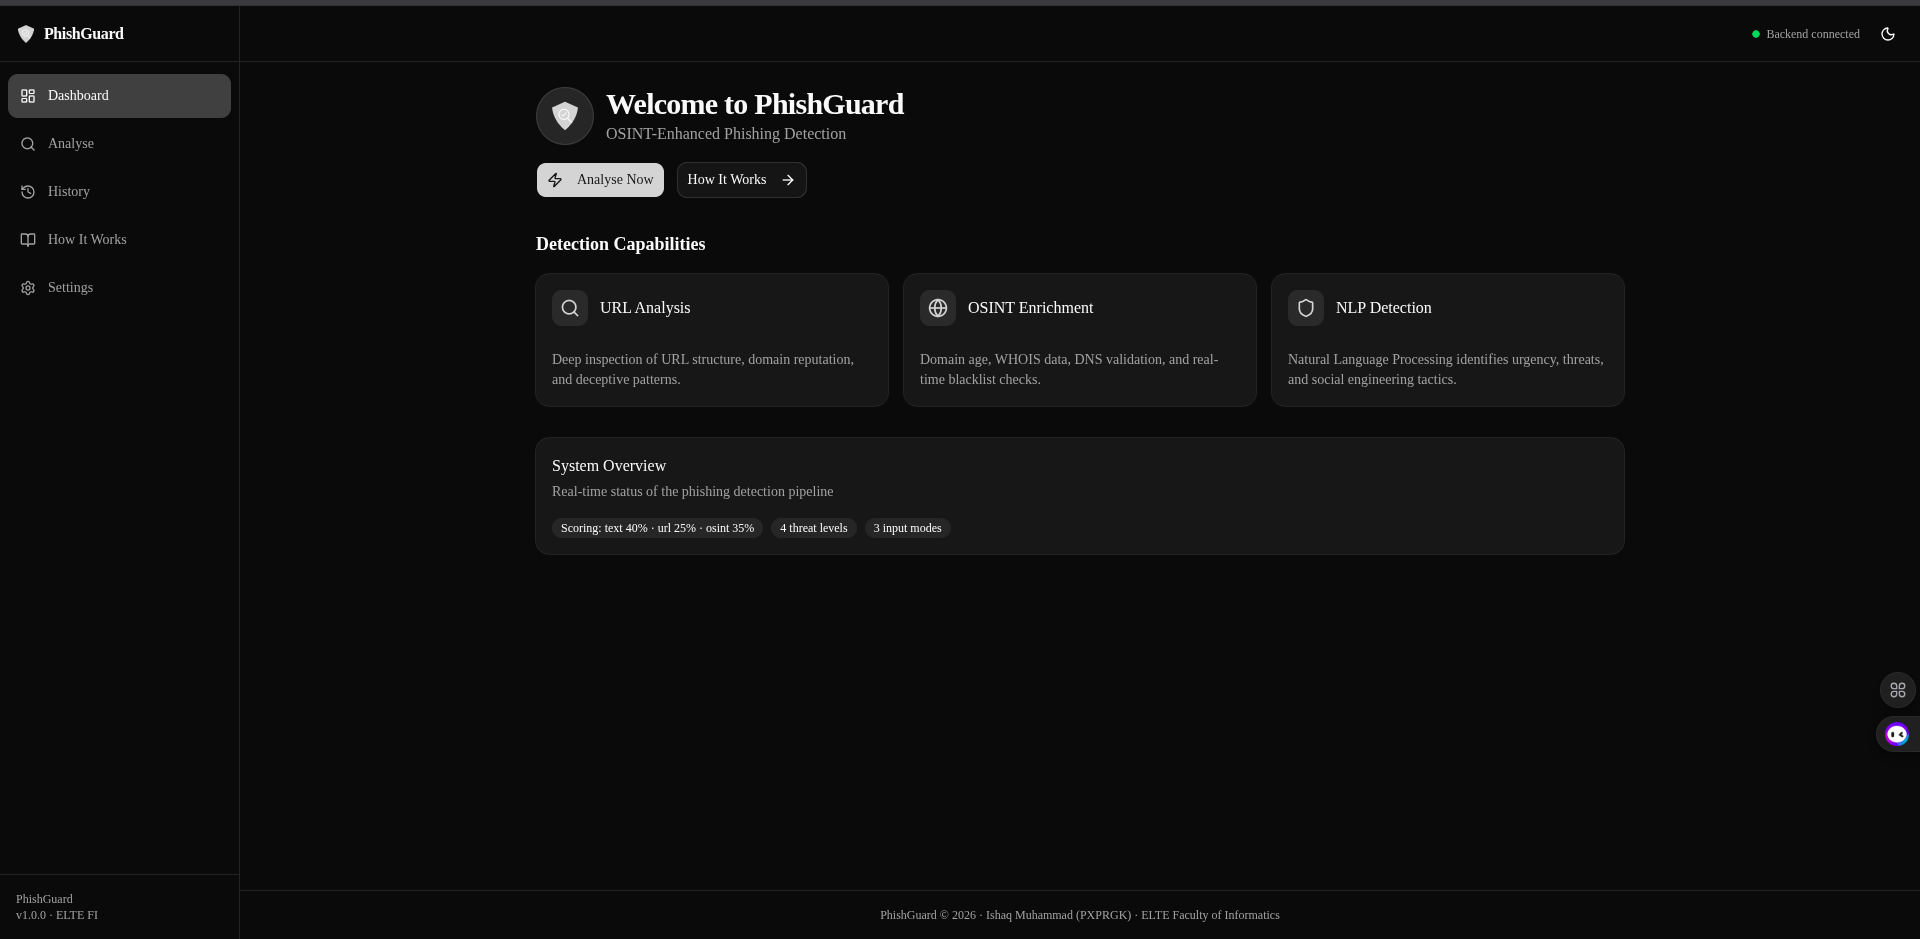
\includegraphics[width=0.85\linewidth,height=0.65\textheight,keepaspectratio]{images/dashboard.png}
\caption{Figure 2.1: The PhishGuard Next.js Web Application Dashboard}
\end{figure}

\subsubsection{Component Architecture and
Styling}\label{component-architecture-and-styling}

The frontend employs a rigorous component-driven design methodology. The
visual aesthetic and layout are strictly managed using Tailwind CSS v4,
a utility-first CSS framework that allows for rapid styling directly
within the component markup.

For complex, interactive UI elements, the project leverages the
\texttt{shadcn} UI library alongside \texttt{@base-ui/react}. These
libraries provide accessible, unstyled components that are seamlessly
integrated with the Tailwind configuration, ensuring a consistent design
language across the application while adhering to web accessibility
guidelines.

\subsubsection{Data Visualization and
Animation}\label{data-visualization-and-animation}

To effectively communicate the complex risk metrics and threat
intelligence data returned by the backend API, the frontend incorporates
the \texttt{recharts} library for data visualization. This library
facilitates the creation of responsive, interactive charts that
illustrate risk scores, temporal data (such as domain age), and
historical analysis trends.

User experience is further enhanced through subtle animations
implemented using the \texttt{motion} (Framer Motion) library. These
animations provide visual feedback during asynchronous state
transitions, such as when waiting for the backend API to complete a
comprehensive URL analysis. Iconography is provided by
\texttt{lucide-react}, ensuring a modern and lightweight visual
presentation.

\begin{figure}
\centering
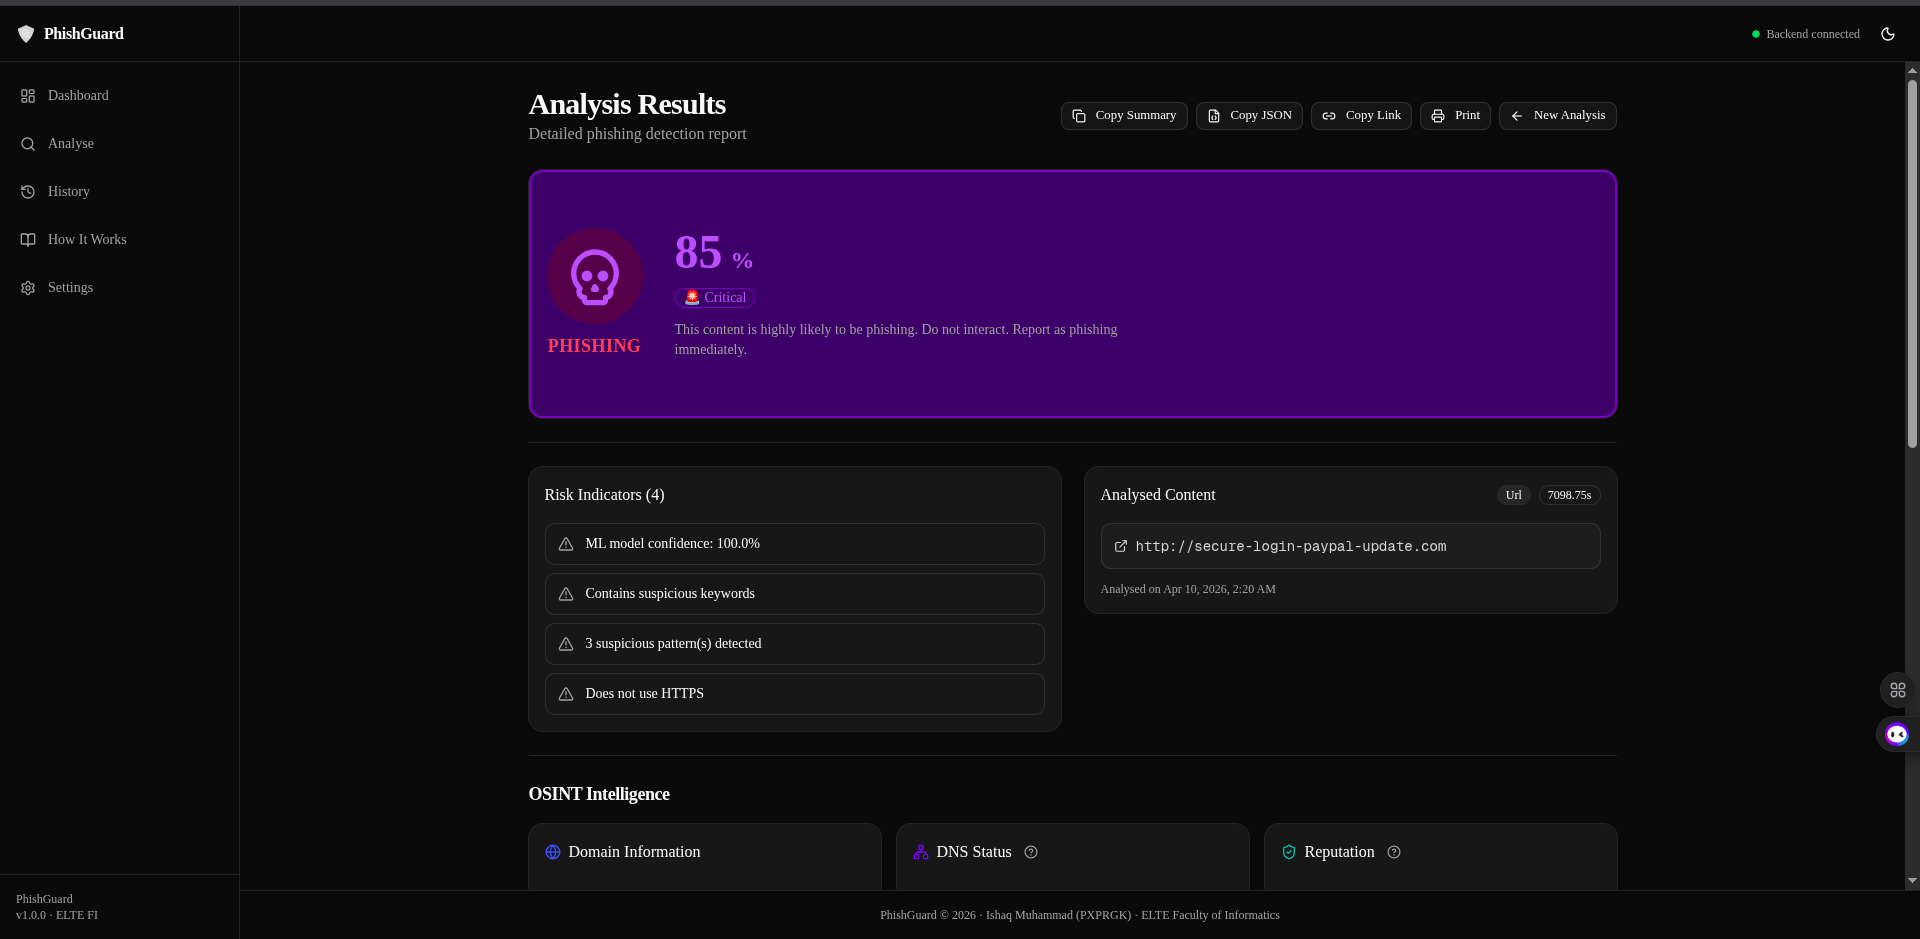
\includegraphics[width=0.85\linewidth,height=0.65\textheight,keepaspectratio]{images/result.png}
\caption{Figure 2.2: Threat Analysis Results showing the interactive
threat gauge}
\end{figure}

